\begin{figure}[h]
	\centering
	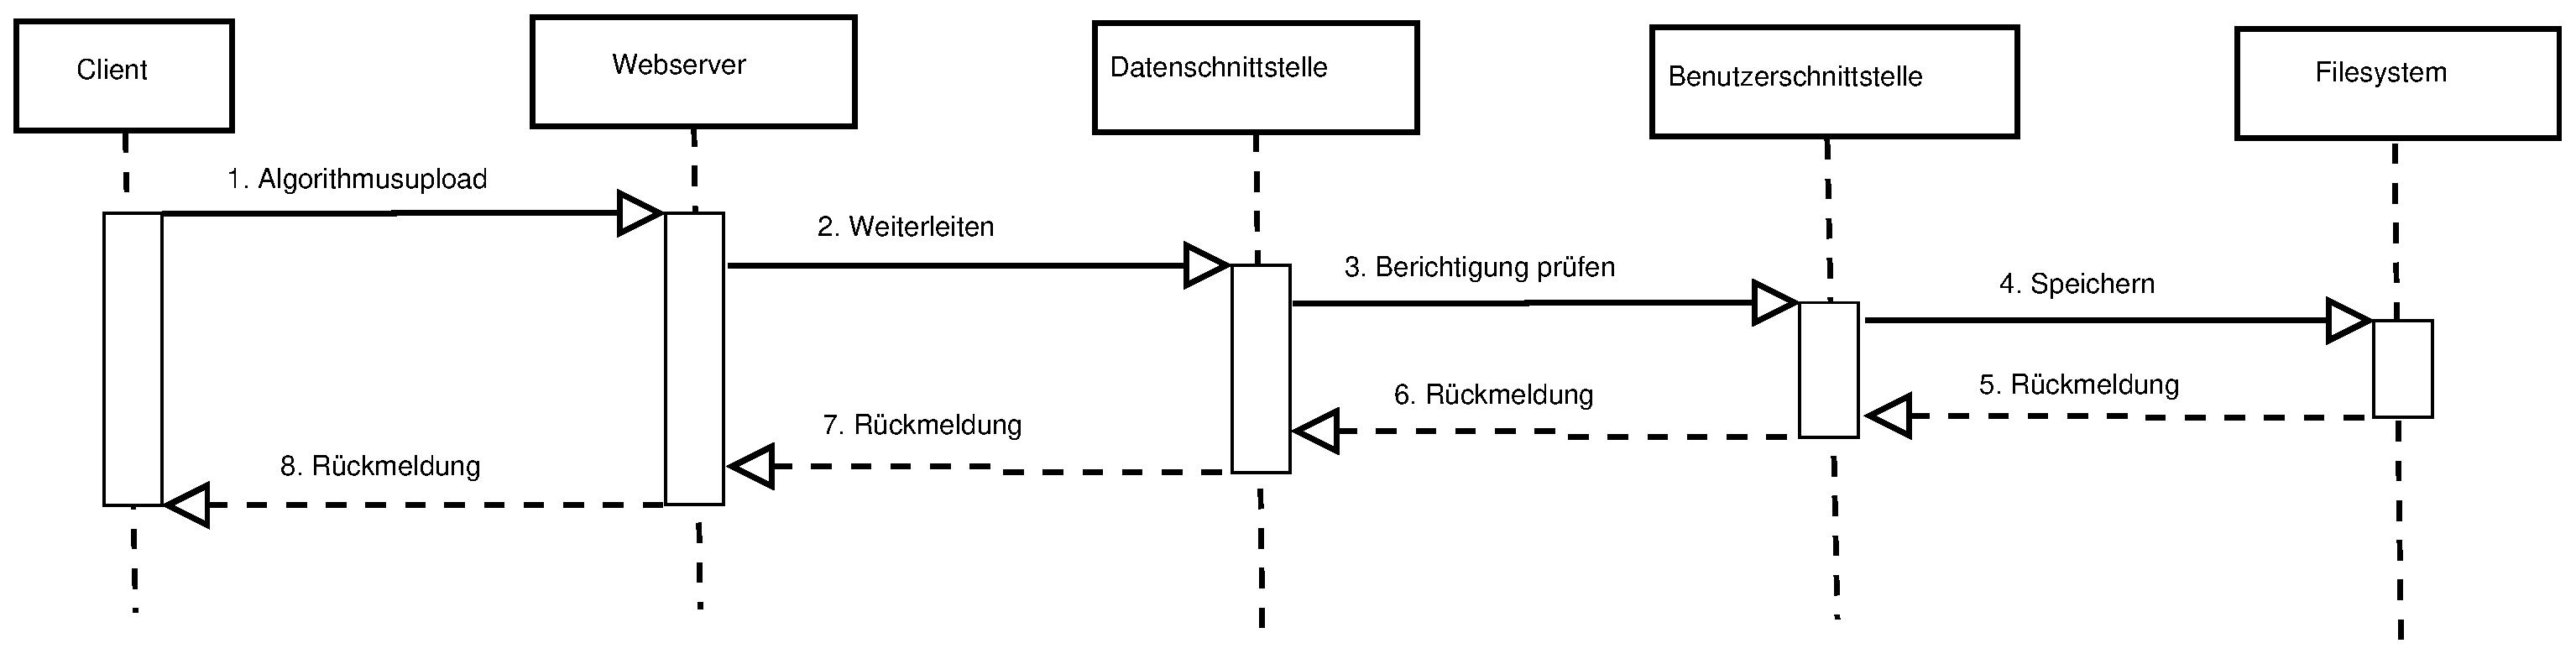
\includegraphics[width=1.0\linewidth]{Grafik/Diagramm/Szenarios/Algorithmus.eps}
	\caption[]{Upload eines Algorithmus}
\end{figure}

\noindent Der Nutzer schickt eine Anfrage zum Upload eines Algorithmus an den Webserver. Dieser delegiert die Nachfrage an die Datenschnittstelle, die diese ihrerseits an die Benutzerschnittstelle zustellt. Dort wird geprüft ob der Nutzer eine Berechtigung zum Upload eines Algorithmus hat, sprich ob er auf dem System registriert ist oder nicht. Sollte er die erforderlichen Kriterien erfüllen, so wird dem Admin der Algorithmus per E-Mail zugestellt und der Benutzer wird über die erfolgreiche Zustellung informiert. Nach Prüfung der übermittelten Daten kann der Admin diese in das Filesystem des Systems integrieren.